\scanpage{116}
% archive sheet number: 115

\uline{Chapitre} 1\qquad Généralités sur les $\otimes$-catégories.

\margin{\handwritten{\deleted{\unsure{catégories} \illegible{1} \unsure{exemples}}\par
\textcircled{1} produit tens. de modules\par
\textcircled{2} catégorie avec produits cart.\par
\textcircled{3} \unsure{torseurs} sous faisceau abélien\par
\textcircled{4} familles de \unsure{modules} \unsure{indexés} par \unsure{groupe}\par
\textcircled{5} espace des lacets d'un espace \fbox{topologique}}}

\uline{Par}.0: Lois $\otimes$ sur une catégorie: exemples divers ....

\uline{Par}.1 \deleted{Les données} Contraintes pour une loi $\otimes$ .

1.1. Associativité.

1.2. Commutativité.

1.3. Unités.

1.4. $\underline{\mathrm{Hom}}(X,Y),\ \underline{\mathrm{Moh}}(Y,X)$\handwritten{;} \handwritten{\deleted{$\unsure{X^\vee}$}} .

\inserted{\handwritten{\figure{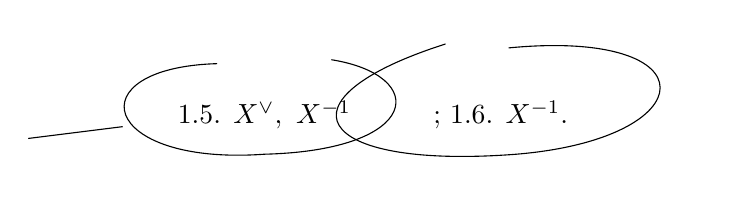
\begin{tikzpicture}[x=1cm,y=1cm]
\node at (0,0) {1.5. $X^\vee,\ \unsure{X^{-1}}$};
\node at (3,0) {; \deleted{\unsure{1.6.}} $X^{-1}$.};
\draw (-3,-.3) -- (-1.8,-.15);
\draw (-.6,.65) .. controls (-2.4,.6) and (-2.1,-.65) .. (0,-.5) .. controls (2,-.45) and (2.1,.5) .. (.85,.7);
\draw (2.3,.9) .. controls (.1,.2) and (.6,-.7) .. (3.2,-.5) .. controls (5.6,-.3) and (5.7,1.1) .. (3.1,.85);
\end{tikzpicture}}}}

\inserted{\handwritten{1.6. Cas des exemples du Par.0}}

\uline{Par}.2\qquad Compatibilités entre contraintes. \handwritten{(Toutes les \inserted{compatibilités entre} contraintes sont satisfaites, quand elles ont un sens, dans les exemples du par.0)}

1.1. Associativité et commutativité.

1.2. Commutativité et unité.

1.3. Associativité et unité.

1.4. \uline{Hom}, \uline{Moh} et associativité: formules de Cartan.

1.5. \uline{Hom} et commutativité (on a alors $\underline{\mathrm{Hom}}\inserted{\handwritten{(X,Y)}}\handwritten{\simeq}\underline{\mathrm{Moh}}\handwritten{(Y,X)}$\handwritten{)}.\handwritten{---}

\inserted{\handwritten{\deleted{(Lois $\otimes$ rigides)}}}

1.6. \uline{Hom} et unité : définition de $X^{\handwritten{\vee}}$ (pour loi commutative seulement ?).\margin{\figure{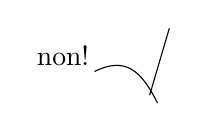
\begin{tikzpicture}[baseline]\node at (0,.4) {\handwritten{\uline{non!}}};\draw (.4,.2) .. controls (.8,.4) and (1,.2) .. (1.2,-.2);\draw (1.1,-.1)--(1.35,.75);\end{tikzpicture}}}

1.7. \inserted{\handwritten{\uline{Lois $\otimes$ rigides.}}} \handwritten{(}Formalisme des traces (cas \deleted{\illegible{1}} d'isomorphie $X^{\handwritten{\vee}}\otimes Y\handwritten{\simeq}\underline{\mathrm{Hom}}(X,Y)$).\handwritten{; rang d'un objet.}

\inserted{\handwritten{\uline{Par}.3}} \deleted{1.8.} Formes normales de multifoncteurs composés. \handwritten{\deleted{(\unsure{après le|pour le} \unsure{§} \uuline{\unsure{suivant}})}}

\uline{Par} \deleted{3}\handwritten{4}.\qquad $\otimes$-foncteurs.

\deleted{3}\handwritten{4}.1. Théorie sans contraintes: définition des $\otimes$-foncteurs, composition, morphismes de $\otimes$-foncteurs.

\deleted{3}\handwritten{4}.2. Compatibilité d'un $\otimes$-foncteur avec des contraintes: associativité et commutativité\handwritten{!}

\deleted{3}\handwritten{4}.3. Compatibilité avec des contraintes: unité.

\deleted{3}\handwritten{4}.4. Compatibilité avec des contraintes: \uline{Hom}, \uline{Moh}, \handwritten{$X^\vee,X^{-1}$ ---}

\inserted{\handwritten{4.5. Objets quasi-inversibles, et \deleted{\unsure{agrandissement} de \unsure{catégories}} \inserted{calcul} des fractions....}}

\uline{Par}. \unsure{4|5}.\qquad \uline{Exemples typiques:}\deleted{\illegible{1}} $\otimes$-\uline{catégories}\handwritten{\uline{définies par des bigèbres}.}

\inserted{\handwritten{5.0. $\otimes$-Catégories: (catégories additives, avec $\otimes$ biadditif, ass. comm. unit. \deleted{\unsure{avec}} \unsure{Gros} méc.\ \uline{$\unsure{\mathrm{Huy}|\mathrm{Hom}}$}).}}

\deleted{4}\handwritten{5}.1. Modules sur une bigèbre.

\deleted{4}\handwritten{5}.2. Comodules sur une bigèbre.

\deleted{4}\handwritten{5}.3. Dualité entre les deux notions: première manière (imparfaite).

\deleted{4}\handwritten{5}.4. Dualité entre les deux notions: seconde manière, formelle (via \deleted{\unsure{notions}} notions d'algèbre dans une $\otimes$-catégorie ).

\inserted{\handwritten{5.5. Modules mixtes (co + ordinaire) sur une bigèbre}}
